% !TeX root = main.tex
\section{Results}
\label{sec:findings}
This section presents the study's descriptive and inferential statistics results, followed by a discussion of the findings.

The results of descriptive statistics revealed that 9\% of the participants rated extraversion, 14\% rated neuroticism, 17\% rated openness to experience, 28\% rated agreeableness, and 32\% rated conscientiousness as their dominant personality traits. Table \ref{tab:correl} shows the pearson's correlations between the big-five personality traits. 

\begin{table}[h]
  \centering
  \caption{Correlations between the Big-Five Traits\label{tab:correl}}
  \vspace{-12pt}
  \begin{tabular}{p{3cm}rrrrr}
    \toprule
    Trait & N & E & O & A & C \\\midrule
    Neuroticism (N) & 1.00 & -0.35 & 0.00 & -0.09 & -0.48 \\
    Extraversion (E) & -0.35 & 1.00 & 0.17 & 0.05 &	0.22 \\
    Openness (O) & 0.00 & 0.17 & 1.00 &	0.15 & -0.07 \\
    Agreeableness (A) & -0.09 &	0.05 & 0.15 & 1.00 & 0.43 \\ 
    Conscientiousness (C) & -0.48 & 0.22 & -0.07 &	0.43 &	1.00  \\\bottomrule
  \end{tabular}\vspace{-8pt}
\end{table}

Additionally, utilizing the plagiarism scores obtained from MOSS for both assignments, students were categorized into plagiarism levels according to the criteria outlined by the University Grants Commission (UGC) \cite{UGCPlagiarism}, a statutory body overseeing higher education in India. The outcomes are detailed in table \ref{tab:levelsPlagiarism}.


\begin{table}[h]
  \centering
  \caption{Percentage of students (out of N=105) falling in each Levels of Plagiarism \label{tab:levelsPlagiarism}}
  \vspace{-12pt}
  \begin{tabular}{p{1cm}p{2cm}rr}
    \toprule
    Level & Similarity \% & Assignment 1 & Assignment 2 \\\midrule
    Level 0 & Less than 10\% & 44.76\% & 40.95\% \\
    Level 1 & 10\% to 40\% & 27.51\% & 40.00\%  \\
    Level 2 & 41\% to 60\% & 14.28\% & 7.61\% \\
    Level 3 & More than 60\% &13.33\% & 11.42\% \\ \bottomrule
  \end{tabular}\vspace{-8pt}
\end{table}

\subsection{Influence of Big-Five traits on Plagiarism}

One of the linear multiple regression assumptions is that the independent variables must not exhibit high (>5) multicollinearity. The multicollinearity between the five personality traits was tested using the variance inflation factor (VIF) and shown in Table \ref{tab:VIF}. All the VIF values were less than 5, indicating that multiple linear regression can be performed. 

\begin{table}[h]
  \centering
  \caption{Big-Five traits and their VIF\label{tab:VIF}}
    \vspace{-12pt}
  \begin{tabular}{p{2cm}r}
    \toprule
    Trait & VIF Value \\\midrule
    Neuroticism & 1.46 \\
    Extraversion & 1.20 \\
    Openness & 1.10\\
    Agreeableness & 1.33 \\ 
    Conscientiousness & 1.70  \\\bottomrule
  \end{tabular}\vspace{-4pt}
\end{table}

Multiple linear regression analyses were conducted, with the big-five personality traits serving as the independent variables and the plagiarism score as the dependent variable for both assignments. The ordinary least squares (OLS) method, a statistical technique used to estimate the relationship between independent and dependent variables, was utilized for the analysis. The dependent variable was plagiarism score and the independent variables were the personality traits. The outcomes are displayed in Table \ref{tab:assign1Regression} and Table \ref{tab:assign2Regression}. $\beta$ Coef indicates the change in the dependent variable for a one-unit change in the independent variable, Std Err measures the variability or dispersion of the beta coefficient, \textit{t} is the ratio of the beta coefficient to its standard error. p-value denotes the level of significance with an asterisk (*) for p < 0.05 and a double asterisk (**) for p < 0.01.

\begin{table}[H]
  \centering
  \caption{Regression analysis on Assignment 1 with $R^2$=0.106\\\label{tab:assign1Regression}}
    \vspace{-12pt}
  \begin{tabular}{p{2.5cm}rrrr}
    \toprule
    Trait & $\beta$ Coef & Std Err & \textit{t} & \textit{p}\\\midrule
    Agreeableness & 0.3489 & 0.243 & 1.434 & 0.155 \\
    Openness & -0.3401 & 0.256 & -1.328 & 0.187 \\
    Neuroticism & -0.1314 & 0.197 & -0.666 & 0.507 \\
    Extraversion & 0.6078 & 0.216 & 2.809 & 0.006** \\
    Conscientiousness & -0.2667 & 0.239 & -1.114 & 0.026* \\\bottomrule
  \end{tabular}\vspace{-12pt}
\end{table}

\begin{table}[H]
  \centering
  \caption{Regression analysis on Assignment 2 with $R^2$=0.128\\\label{tab:assign2Regression}}
    \vspace{-12pt}
  \begin{tabular}{p{2.5cm}rrrr}
    \toprule
    Trait & $\beta$ Coef & Std Err & \textit{t} & \textit{p}\\\midrule
    Agreeableness & 0.3291 & 0.211 & 1.561 & 0.122 \\
    Openness & -0.3750 & 0.222 & -1.691 & 0.094\\
    Neuroticism & -0.2919 & 0.171 & -1.708 &  0.091\\
    Extraversion & 0.4394 & 0.187 & 2.344 & 0.021*\\
    Conscientiousness & -0.5541 & 0.207 & -2.673 & 0.009**\\\bottomrule
  \end{tabular}\vspace{-8pt}
\end{table}

Based on the findings from both assignments, irrespective of the actual coefficient values, it is apparent that extraversion exhibits a positive association with plagiarism (\textit{p}<0.05), while conscientiousness demonstrates a negative association with plagiarism (\textit{p}<0.05). However, the other personality traits are not statistically significant (\textit{p} values greater than 0.05).

\vspace{8pt}
\begin{mdframed}
\textbf{\textit{RQ1 Answer:}} Extraversion and conscientiousness traits influence plagiarism, with extraversion positively associated and conscientiousness negatively associated. The other three traits do not show a significant influence on plagiarism. 
\end{mdframed}
\vspace{8pt}

Some of these observations align with those reported in the literature, as illustrated in Table \ref{tab:litSUmmary}. For example, the lack of significance for openness to experience and neuroticism, as well as the negative association of conscientiousness with plagiarism, are consistent with the findings of Wilks et al. \cite{Wilks2016-WILPTA-3} and Giluk et al. \cite{Giluk2015BigFP}. 

However, in our study, extraversion demonstrates a positive association with plagiarism, consistent with the findings of Bhutto et al. \cite{Bhutto2019ACS} as shown in Fig \ref{fig:personalityAndPlagiarism}. 

\begin{figure}[H]
  \centering
  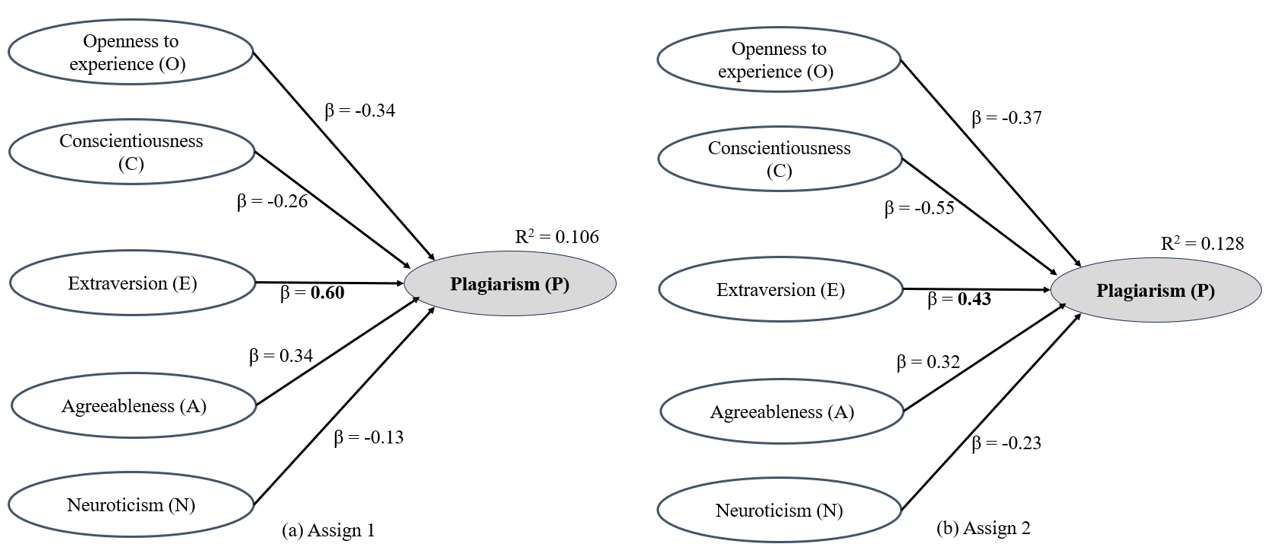
\includegraphics[width=\columnwidth]{1.png}
  \caption{The relationship between the big five traits and plagiarism in (a) Assign 1 and (b) Assign 2}
  \Description{In both of them, extroversion has a positive influence and openness to experience, and conscientiousness and neuroticism negatively influence plagiarism scores.}
  \label{fig:personalityAndPlagiarism}
\end{figure}

\subsection{Student behavior after sensitization via Honor Pledge }

The normality of plagiarism scores for Assignment 1 and Assignment 2 was assessed using histograms and the Shapiro-Wilk test, confirming their normal distribution. Our null hypothesis suggested that there would be no change in the mean percentage of similar lines of code after students were sensitized through an honor pledge for the second programming assignment. Given that we were comparing scores from the same students pre-intervention (Assignment 1 plagiarism scores) (N=105, Mean=23.45; SD=26.25) and post-intervention (Assignment 2 plagiarism scores) (N=105, Mean=21.23; SD=23.02), we conducted a paired t-test, \textit{t}(105) = 0.89, \emph{p} = 0.374, d = 0.0899. Here, the intervention refers to the earlier honor pledge (Sec 4). As p>0.05, we did not reject the null hypothesis. 

As depicted in Table \ref{tab:levelsPlagiarism}, there was a slight decrease in the percentage of students classified in levels 2 and 3 of plagiarism after the intervention. While there was a marginal decline in the average plagiarism percentage from Assignment 1 to Assignment 2 (from 23.44\% to 21.22\%), the effect size computed using Cohen's d was minimal (d=0.08). 

\vspace{4pt}
\begin{mdframed}
\textbf{\textit{RQ2 Answer:}} Our findings suggest that while educating students about plagiarism and collusion via an honor pledge may have some effect, its effectiveness in reducing plagiarism and collusion in programming assignments is limited as long as opportunities and pressure to engage in such behavior persist.
\end{mdframed}
\vspace{4pt}

% WORK FROM HERE ....

We specifically conducted the test for students who were involved in plagiarism and/or collusion in Assignment 1, identified by a similarity score greater than 10\% (those falling into levels 1, 2, and 3 in Assignment 1, as shown in Table \ref{tab:levelsPlagiarism}). This allowed us to evaluate whether the intervention benefited students who engaged in such academic misconduct in Assignment 1, as they are the ones who might benefit most from such intervention. The paired sample t-test revealed a significant difference: the percentage of similarity score in Assignment 1 (N=58, Mean=41.73, SD=21.44) was notably higher than in Assignment 2 (N=58, Mean=28.92, SD=26.27); t(58)=3.52, p=0.0008, d=0.53 (moderate effect). Similarly, when the t-test was performed only on those who did not plagiarize and/or were involved in collusion, i.e., those whose similarity score was <10\% in assignment 1, p<0.001, suggesting that we could reject the null hypothesis. 




In both assignments, the students were not provided explicit information regarding the plagiarism checks that would be conducted using MOSS on their solutions. Students perceived that there was still an opportunity for plagiarism.
\color{blue}(Our results show that sensitizing students about plagiarism does not reduce plagiarism. Students continue to plagiarize through collusion as long as they perceive that an opportunity exists.)\color{black}
Consequently, the impact of the honor pledge on reducing plagiarism was perceived as weak.


\section{Discussion} \label{sec:discuss}

Our findings indicate that individuals with high extraversion scores demonstrate a greater tendency to engage in collusion to perform better in programming assignments. This propensity aligns with the Fraud Triangle model, where heightened extraversion fosters sociability and potentially larger social circles and friends, thereby increasing opportunities for collusion. Moreover, extroverted individuals may find it easier to rationalize their actions as commonplace due to their sociable nature.

The correlation between extraversion and plagiarism in India's academic environment can be understood within the \textit{pressure} aspect of the fraud triangle model. In this model, pressure refers to the internal or external forces that compel individuals to engage in misconduct. In Indian society, there is often a strong emphasis on competitiveness and achievement, particularly in academic settings where grades and academic success are highly valued. For instance, prestigious institutions like the IITs, which are top-ranked according to the National Institutional Ranking Framework (NIRF), the official framework for ranking higher education institutes across India \footnote{\url{https://www.nirfindia.org/2023/EngineeringRanking.html}}, receive applications from over one million students every year for a limited number of seats, typically around 10,000. This intense competition and pressure to excel start early, with students enrolling in specialized coaching institutes for exam preparation as young as ten years old \cite{IITPrepMenace}. 

Furthermore, the pressure to obtain employment is aggravated by the harsh realities of the job market. India has approximately 2 million computer science students, with ongoing concerns regarding employability rates, which can drop to as low as below 25\% \cite{UnemploymentIndia, NAIR2020831}. As a result, a significant number of graduates encounter challenges in securing suitable job opportunities. The pressure to succeed in this fiercely competitive environment and pressure stemming from societal expectations, family aspirations, and the intense competition for limited opportunities, creates a potent force that may drive individuals to resort to unethical practices like plagiarism and collusion to gain a competitive edge. 

This environment fosters a mentality of optimizing results by any means necessary. Thus, the propensity for plagiarism is driven more by opportunity than rationale, as students feel pressured to perform. 

Extraverted individuals, characterized by their sociability, assertiveness, and tendency to seek stimulation, may be more inclined to engage in behaviors to achieve success, even if it involves unethical practices such as plagiarism and collusion.

Furthermore, the pressure to excel academically and limited awareness or enforcement of academic integrity policies may create an environment where extraverted students feel more comfortable engaging in plagiarism to achieve their goals. These factors collectively suggest that the positive influence of extraversion on plagiarism in India may stem from a combination of cultural, societal, and educational factors that shape individuals' attitudes and behaviors toward academic integrity.
\color{blue}(Our results also show that more conscientious individuals are less likely to plagiarize. This can also be explained using the Fraud triangle model. A conscientious individual might be less likely to make use of the opportunity to indulge in plagiarism and rationalize the behaviour. )\color{black}